\documentclass[11pt]{beamer}
\usetheme{Warsaw}
\usepackage[utf8]{inputenc}
\usepackage[french]{babel}
%\usepackage[T1]{fontenc}
\usepackage{amsmath}
\usepackage{amsfonts}
\usepackage{amssymb}
\usepackage{listings}
\usepackage{color}
\definecolor{lightgray}{rgb}{.9,.9,.9}
\definecolor{darkgray}{rgb}{.4,.4,.4}
\definecolor{purple}{rgb}{0.65, 0.12, 0.82}
\lstdefinelanguage{JavaScript}{
  keywords={do, if, in, for, let, new, try, var, case, else, enum, eval, null, this, true, void, with, await, break, catch, class, const, false, super, throw, while, yield, delete, export, import, public, return, static, switch, typeof, default, extends, finally, package, private, continue, debugger, function, arguments, interface, protected, implements, instanceof},
  morecomment=[l]{//},
  morecomment=[s]{/*}{*/},
  morestring=[b]',
  morestring=[b]",
  ndkeywords={class, export, boolean, throw, implements, import, this},
  keywordstyle=\color{blue}\bfseries,
  ndkeywordstyle=\color{darkgray}\bfseries,
  identifierstyle=\color{black},
  commentstyle=\color{purple}\ttfamily,
  stringstyle=\color{red}\ttfamily,
  sensitive=true
}

\lstset{
   language=JavaScript,
   backgroundcolor=\color{lightgray},
   extendedchars=true,
   basicstyle=\footnotesize\ttfamily,
   showstringspaces=false,
   showspaces=false,
   numbers=left,
   numberstyle=\footnotesize,
   numbersep=9pt,
   tabsize=2,
   breaklines=true,
   showtabs=false,
   captionpos=b
}

\lstset{literate=
  {á}{{\'a}}1 {é}{{\'e}}1 {í}{{\'i}}1 {ó}{{\'o}}1 {ú}{{\'u}}1
  {Á}{{\'A}}1 {É}{{\'E}}1 {Í}{{\'I}}1 {Ó}{{\'O}}1 {Ú}{{\'U}}1
  {à}{{\`a}}1 {è}{{\`e}}1 {ì}{{\`i}}1 {ò}{{\`o}}1 {ù}{{\`u}}1
  {À}{{\`A}}1 {È}{{\'E}}1 {Ì}{{\`I}}1 {Ò}{{\`O}}1 {Ù}{{\`U}}1
  {ä}{{\"a}}1 {ë}{{\"e}}1 {ï}{{\"i}}1 {ö}{{\"o}}1 {ü}{{\"u}}1
  {Ä}{{\"A}}1 {Ë}{{\"E}}1 {Ï}{{\"I}}1 {Ö}{{\"O}}1 {Ü}{{\"U}}1
  {â}{{\^a}}1 {ê}{{\^e}}1 {î}{{\^i}}1 {ô}{{\^o}}1 {û}{{\^u}}1
  {Â}{{\^A}}1 {Ê}{{\^E}}1 {Î}{{\^I}}1 {Ô}{{\^O}}1 {Û}{{\^U}}1
  {œ}{{\oe}}1 {Œ}{{\OE}}1 {æ}{{\ae}}1 {Æ}{{\AE}}1 {ß}{{\ss}}1
  {ű}{{\H{u}}}1 {Ű}{{\H{U}}}1 {ő}{{\H{o}}}1 {Ő}{{\H{O}}}1
  {ç}{{\c c}}1 {Ç}{{\c C}}1 {ø}{{\o}}1 {å}{{\r a}}1 {Å}{{\r A}}1
  {€}{{\euro}}1 {£}{{\pounds}}1 {«}{{\guillemotleft}}1
  {»}{{\guillemotright}}1 {ñ}{{\~n}}1 {Ñ}{{\~N}}1 {¿}{{?`}}1
}

\author{Niels Lachat, \\ Mentor : Patrick Rickli}
\title{Soutenance : \\ De Révolution à Evolution}
%\setbeamercovered{transparent} 
\setbeamertemplate{navigation symbols}{} 
\logo{
\includegraphics[scale=.1]{../../documents/images/logo}} 
\institute{Lycée Denis-de-Rougemont} 
\date{17 mai 2018} 
%\subject{} 

\newcommand{\pauseditemize}{\pause \begin{itemize}[<+->]}


\begin{document}

\begin{frame}
\titlepage
\end{frame}

\begin{frame}
\tableofcontents
\end{frame}

\section{Choix du sujet}

\begin{frame}{Choix du sujet}

\pauseditemize
	\item Intérêt pour l'informatique et les jeux vidéos
	\item Ecosia $\Rightarrow$ on peut changer le monde réel grâce au monde virtuel
	\begin{center}
		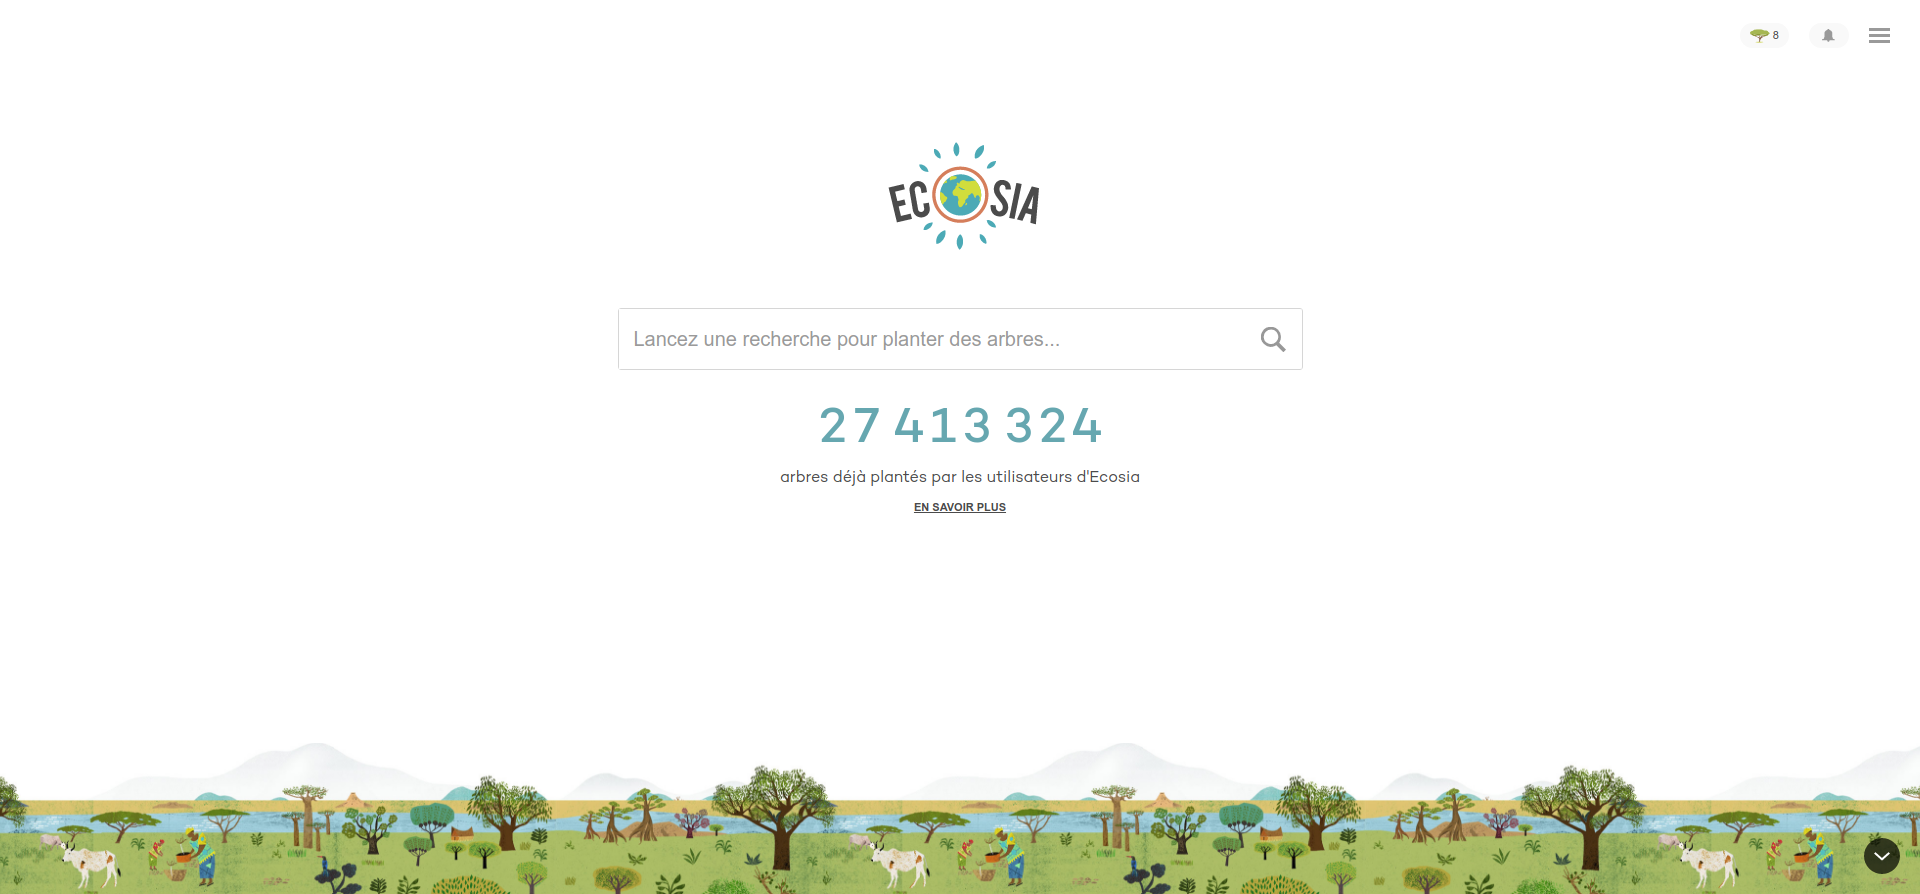
\includegraphics[scale=.1]{../images/ecosia}
	\end{center}
\end{itemize}

\end{frame}


\section{Objectifs initiaux}

\begin{frame}{Objectifs initiaux}

\pauseditemize
	\item Jeu de gestion avec aspects écologiques
	\item Événements historiques
	\item $\Rightarrow$ Engendre une réflexion
\end{itemize}

\end{frame}

\section{Objectifs finaux}

\begin{frame}{Objectifs finaux}

\pauseditemize
	\item Un aspect de l'écologie: la transition énergétique
	\item Pas d'événements historiques (trop long)
	\item Objectifs du jeu calqués sur l'Accord de Paris sur le climat
\end{itemize}

\end{frame}

\section{Difficultés rencontrées}

\begin{frame}{Difficultés rencontrées}

\pauseditemize
	\item Mise à jour du \textit{Newspaper} (onglets)
	\item Ajustements des valeurs
\end{itemize}

\end{frame}

\section{Codes intéressants pas montrés dans le TM} %ATTENTION : PLURIEL, PAS PLURIEL?

\begin{frame}{poly.js}

\lstinputlisting[language=JavaScript, basicstyle=\tiny, lastline=10]{../../web_src/scripts/utils/poly.js}

\end{frame}

\begin{frame}{Les régions}
Les polygones définissent des régions:
\begin{center} 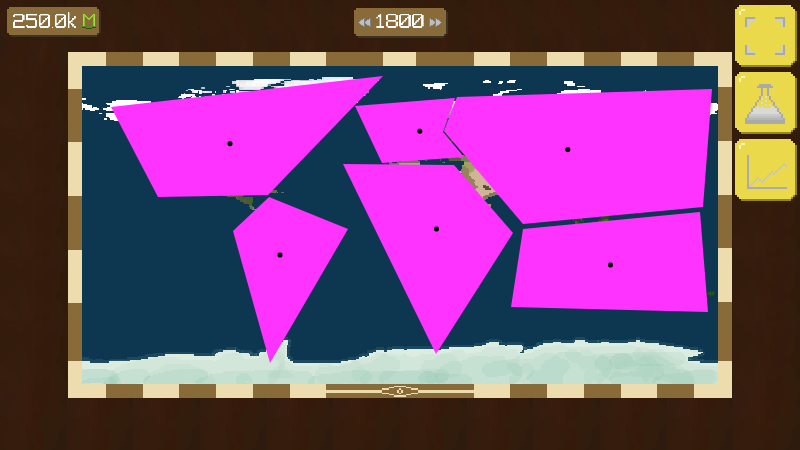
\includegraphics[scale=.3]{../images/regionsPoly} \end{center}
\end{frame}

\begin{frame}{globReg.js}

\lstinputlisting[language=JavaScript, basicstyle=\tiny, firstline=70, lastline=83]{../../web_src/scripts/utils/globReg.js}

\end{frame}

\section{Conclusion}
\subsection{Elements appris durant le TM}

\begin{frame}{ES6}

\begin{center}
	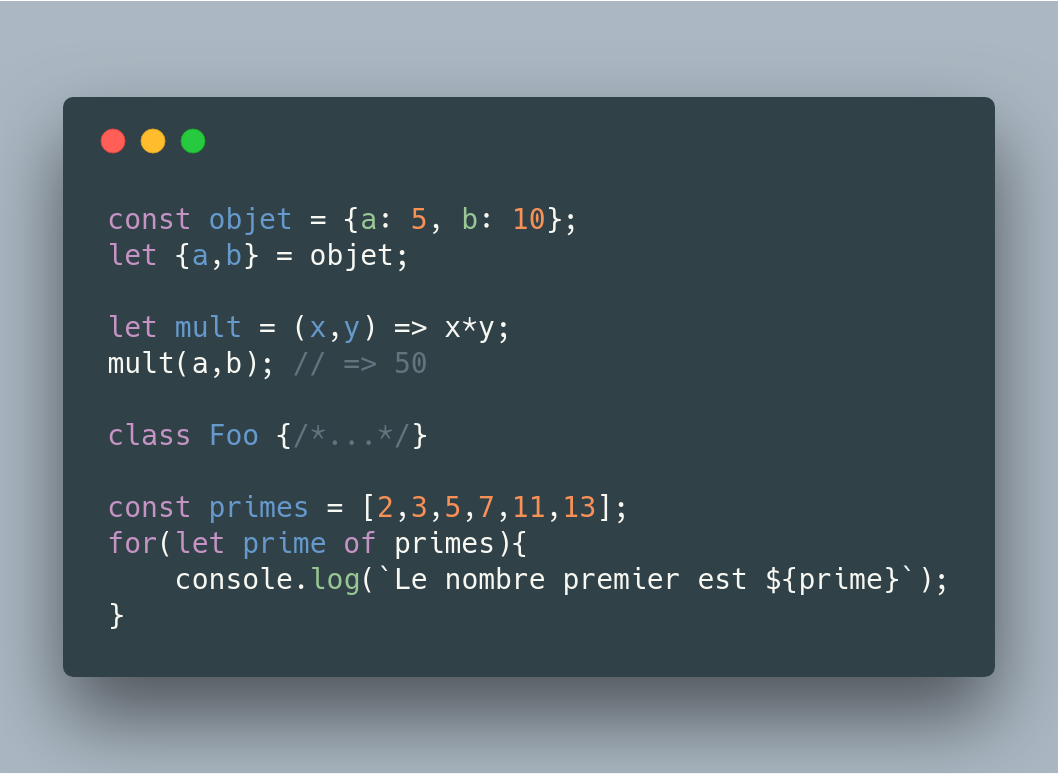
\includegraphics[scale=.2]{../images/es6}
\end{center}

\end{frame}

\begin{frame}{Phaser.js}

\pauseditemize
	\item States, Tweens, Animations, etc\dots
	\item Apprentissage par la documentation
	\item Fonctionnement des librairies open source
\end{itemize}

\end{frame}

\begin{frame}{Latex}
	
\pauseditemize
	\item Travail de maturité, instructions (documentclass : article)
	\item Présentation (documentclass : beamer)
\end{itemize}

\end{frame}

\begin{frame}{Autres}

\pauseditemize
	\item Dessin en 'Pixel Art'
	\item Git \& Github
	\item Organisation de code de taille importante
\end{itemize}

\pause
\begin{center}
	
\includegraphics[scale=.3]{../images/Think-Twice-Code-Once}
\end{center}

\end{frame}

\subsection{Continuation}

\begin{frame}

\pauseditemize
	\item Continuer le jeu (difficulté, musique/sons, histoire/événements historiques, actions écologiques)
	\begin{center} 
		
\includegraphics[scale=.08]{../images/ecoActions} 
	\end{center}
\end{itemize}

\end{frame}

\section{Questions}

\begin{frame}{Questions}
	\begin{center}
	{\LARGE Questions}
	\end{center}
\end{frame}


\end{document}